\chapter{Resolution of the system}

The aim of this chapter is to introduce notation and to present the physical model exposed in the previous chapter, in a more precisely and mathematical form. A briefely overview on the avaible and used iteration algorithms is then treated.

\section{Geometry and boundary conditions}

Consider the stationary form of problem \referenzaeq{eq: full problem}, in order to proceed we have to close the \textit{Poisson equation} and the \textit{Drift Diffusion equation} for electrons and holes with suitable boundary conditions over the domain.

Let us consider the device domain as the union of two open disjoint subsets, $\Omega_{Si}$ (doped silicon part), and $\Omega_{ox}$ (oxide part), such that their intersection $\partial \Omega_{Si} \cap \partial \Omega_{ox} = \Gamma_{int}$ is the interface. The oxide region $\Omega_{ox}$ is assumed to be a perfect insulator so that:

\begin{equation}
\label{eq: hypotesis oxide}
\begin{array}{c}
n = p = 0 \\
\vect{J}_n = \vect{J}_p = \vect{0}

\end{array}
\end{equation}

The device boundary $\partial \Omega$ is divided into two disjoint subsets: $\partial \Omega_{c}$ and $\partial \Omega_{a}$.
The subset $\partial \Omega_{c}$ includes the so called \textit{ohmic contacts}. With ohmic contacts we define every electrical terminal of the device on which the external input voltages are applied. Moreover ohmic contacts are assumed to be \textit{ideal}, they are equipotential surfaces and no voltage drop occurs at the interface between the contact and the neighbouring material. This event is well performed by suitable Dirichlet boundary conditions, therefore in the follow we indicate $\partial \Omega_{c} = \Gamma_D$.

\begin{equation}
\label{eq: dirichlet boundary condition}
\begin{array}{cc}
\varphi = \varphi_D & \\
n = n_D & \psp{10} on \, \Gamma_D .\\
p = p_D & 
\end{array}
\end{equation}

In the case where the neighbouring material is a perfect insulator, hypotesis \referenzaeq{eq: hypotesis oxide} takes in place and therefore no Drift-Diffusion equations are solved, this implies that \referenzaeq{eq: dirichlet boundary condition} reduces to the sole condition on the potential.

\begin{figure}[!b]
\centering
\subfloat[][\label{fig: dop}]
{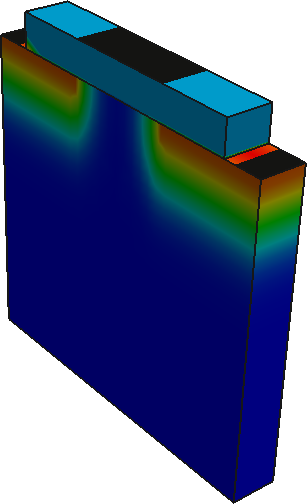
\includegraphics[scale=0.35]{Resolution/MosContacts}}
\psp{30}
\subfloat[][]
{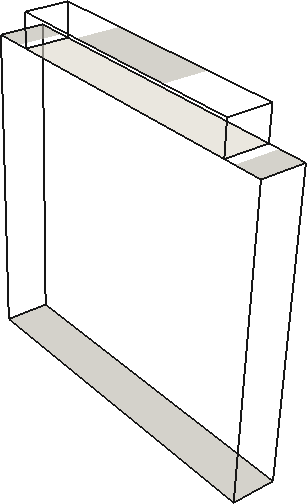
\includegraphics[scale=0.35]{Resolution/MosOnlyContacts}}
\caption{(a) Mos device with net dopant concentration distributed accordingly to a gaussian profile and $\Gamma_D$ colored in black. The oxide layer is colored in light blue. (b) Outline of the Mos device with $\Gamma_{int}$ in light gray. }
\end{figure}

Artificial boundaries ($\partial \Omega_a$) are needed in order to obtain a self-contained simulation domain.  On these boundaries no electric and current flux is exchanged with the surrounding environment, this fact is well performed by homogeneous Neumann boundary condition ($\partial \Omega_a = \Gamma_N$)

\begin{equation}
\label{eq: neumann boundar condition}
\begin{array}{cc}
\vect{D}\cdot \vect{n} = 0 & \\
\vect{J}_n \cdot \vect{n} = 0 & \psp{10} on \, \Gamma_N \\
\vect{J}_p \cdot \vect{n} = 0 & 
\end{array}
\end{equation}

where $\vect{n}$ is the outward unit normal vector defined over $\partial \Omega$. 
As we noted before on $\partial \Omega_{ox} \cap \Gamma_N$ condition \referenzaeq{eq: neumann boundar condition} reduces to the sole one related with the Poisson equation.

Finally when we solve a Drift-Diffusion equation, if $\Omega_{ox} \neq \varnothing$ boundary shape could be change. Although the treatment of boundaries doesn't change if you consider the suitable restrictions and extensions
\begin{equation}
\begin{array}{c}
\Gamma_{D,Si} = \Gamma_D \cap \partial \Omega_{Si} \\
\Gamma_{N,Si} = \Gamma_N \cap \partial \Omega_{Si} \cup \Gamma_{int}.
\end{array}
\end{equation}

In silicon material the ideal condition on contacts is accomplished if both thermodynamical equilibrium and charge neutrality are reached. These two conditions correspond to the following algebraic system for $n_D$ and $p_D$

\begin{equation}
\label{eq: systemo for dirichlet condition}
\left\{
\begin{array}{lcl}
p_Dn_D & = &n_i^2 \\
p_D -n_D +N_D-N_A & = & 0 
\end{array}
\right. .
\end{equation}

Solving \referenzaeq{eq: systemo for dirichlet condition} on $\Gamma_{D,Si}$ we obtain:

\begin{equation}
n_D = \dfrac{D + \sqrt{D^2+4n_i^2}}{2}
\end{equation}
\begin{equation}
p_D = \dfrac{-D + \sqrt{D^2+4n_i^2}}{2}
\end{equation}

where $D := N_D-N_A$ is the net doping concentration. Furthermore  we can approximate that the quasi fermi potential level of silicon at contact is aligend with the external applyed voltage. As a consequence we can easily calculate potential condition on $\Gamma_{D,Si}$ using \referenzaeq{eq: n density mb} and \referenzaeq{eq: p density mb}

\begin{equation}
\varphi_D = \varphi_f + V_{th}ln\left( \dfrac{n_D}{n_i} \right) = \varphi_f - V_{th}ln\left( \dfrac{p_D}{n_i} \right)
\end{equation}

where $\varphi_f = - E_f / q$ is the unique quasi fermi potential level defined on contacts. When $\Omega_{ox} \neq \varnothing$ we set $\varphi_D$ equal to the external applyed voltage on $\Gamma_D / \Gamma_{D,Si}$.


As we conveyed the boundary conditions, we are able to write in the closed way the stationary form of problem \referenzaeq{eq: full problem} as follows:
 

\begin{equation}
\label{eq: system closed}
\begin{array}{rcll}
- \Delta \epsilon \varphi - q(p-n) & =  & qD & in \, \Omega = \Omega_{ox} \cup \Omega_{Si}\\
\varphi & = & \varphi_D & on \, \Gamma_D \\
\nabla \varphi \cdot \vect{n} & = & 0 & on \, \Gamma_N 
\\
\\
\nabla \cdot ( q\mu_n n \nabla \varphi - qD_n \nabla n ) & = & - qR & in \, \Omega_{Si}\\
n & = & n_D & on \, \Gamma_{D,Si} \\
\nabla n \cdot \vect{n} & = & 0 & on \, \Gamma_{N,Si}
\\
\\
\nabla \cdot (- q\mu_p p \nabla \varphi - qD_p \nabla p )& = & -qR& in \, \Omega_{Si}\\
p & = & p_D & on \, \Gamma_{D,Si} \\
\nabla p \cdot \vect{n} & = & 0 & on \, \Gamma_{N,Si}
\end{array}
\end{equation}

The high coupled nonlinear nature of system	\referenzaeq{eq: system closed} makes an analytical treatment very difficult, if not even impossible. For this reason, numerical schemes must be used to compute an approximate solution. 


\section{Iteration algorithms}

 The most used algorithms are \textit{the fully coupled Newton's method} and \textit{the decoupled Gummel map}. First of all we introduce a more compact form of \referenzaeq{eq: system closed}:

\begin{equation}
\label{eq: abstract problem fully}
\vect{F(U)}=\vect{0}
\end{equation}

where:

\begin{equation}
\label{eq: functional operator}
\vect{U}:=[\varphi,n,p]^T \psp{30} \vect{F(U)}:=\left[ \begin{array}{c}
F_1(\vect{U}) \\
F_2(\vect{U}) \\
F_3(\vect{U})
\end{array}
\right]
\end{equation}

and having set:

\begin{align*}
F_1(\vect{U}) & = \nabla \cdot (-\epsilon \nabla \varphi) - q(p-n+D) \\
F_2(\vect{U}) & = \nabla \cdot ( q\mu_n n \nabla \varphi - qD_n \nabla n )+qR \\
F_3(\vect{U}) & = \nabla \cdot (- q\mu_p p \nabla \varphi - qD_p \nabla p )+qR
\end{align*}

The non linear problem \referenzaeq{eq: abstract problem fully} is the abstract generalization of the search of a zero for a real function $f:\mathbb{R}\rightarrow\mathbb{R}$. Although the vector function $\vect{F}$ is a nonlinear differential operator and the associated problem which we intend to resolve is: given a functional space $V$ and the operator $\vect{F}:V\rightarrow V$, find $\vect{U}\in V$ such that \referenzaeq{eq: abstract problem fully} is satisfied.

In our application, the function space $V$ is tipycally a subset of the Sobolev space  $[H^1(\Omega)]^d$ (in this case with $d$ we intend the number of component of $\vect{F}$). Sobolev spaces are based on the space of square integrable functions on $\Omega$ which reads as follows

\begin{equation}
\label{space: L2}
L^2(\Omega) := \left\{ v : \int_{\Omega} |v|^2 d\,\Omega =||v||^2_{L^2(\Omega)}<+\infty \right\}.
\end{equation}

The general form of a Sobolev space for an integer $m\geq 0$ is

\begin{equation}
\label{space: Hm}
H^m(\Omega) := \left\{ v : D^{\alpha}v\in L^2(\Omega),\forall |\alpha|\leq m \right\}.
\end{equation}

On this space, we shall use the semi-norm

\begin{equation}
\label{eq: semiorm sobolev}
|v|_{m,\Omega}^2 = \sum_{|\alpha|=m} ||D^{\alpha}v||^2_{L^2(\Omega)}
\end{equation}

and the norm

\begin{equation}
\label{eq: norm sobolev}
||v||_{m,\Omega}^2 = \sum_{k\leq m} |D^{\alpha}v|^2_{k,\Omega}
\end{equation}

We shall also need to consider functions that vanish on either the entire or a part of the boundary

\begin{align}
& H^1_0 :=  \left\{   v : v \in H^1(\Omega), v|_{\partial \Omega} = 0\right\} \label{space: h1 zero} \\
& H^1_{0,\Gamma_D} :=  \left\{   v : v \in H^1(\Omega), v|_{\Gamma_D} = 0\right\} \label{space: h1 zero gamma}
\end{align} 

For $v \in H^1_0(\Omega)$ we have the \textit{Poincar\'e inequality}

\begin{equation}
\label{eq: poincarre inequality}
|v|_{0,\Omega} \leq C(\Omega) |v|_{1,\Omega}
\end{equation}

and the seminorm $|\cdot |_{\,\Omega}$ is therefore a norm in $H^1(\Omega)$, equivalent to $||\cdot ||_{1,\Omega}$.

The above setting of function spaces are used widely in the proceeding of this work, especially during the well-posedness analysis of the equations in chapter \ref{chap: finite element}.


\subsection{Abstract Newton's method}

Before introducing the abstract Newton's method we have to define some useful concept.

\begin{Definizione}[Frech\`et differentiable]
Let be $X$ and $Y$ two vector spaces. Given $f,g \in X$ and a functional $F:X\rightarrow Y$, the functional $F$ is Frech\'et differentiable if it exists a linear bounded operator $A_f:X\rightarrow Y$ such that:

\begin{equation}
\lim_{||g||\to 0}\dfrac{||F(f+g)-F(f)-A_f(g)||_Y}{||g||_X} = 0 
\end{equation}

If the limit exists, we write $DF(f)=A_f$ and call it the Frech\'et derivative of $F$ at $f$.
\end{Definizione}


Considering the functional operator \referenzaeq{eq: functional operator} we can easily compute the relative \textit{Jacobian matrix} $\vect{F}'$, whose $(i,j)-th$ entry represents the Frech\'et derivative of the $i-th$ row of the non linear operator with respect to the $j-th$ variable.

\begin{equation}
\vect{F}'_{ij}(\vect{U})[\vect{V}]_j := \lim_{\eta \to 0}\dfrac{F_i(\vect{U}+\eta [\vect{V}]_j)-F_i(\vect{U})}{\eta}  \psp{10} \vect{V} \in V
\end{equation}

where $[\vect{V}]_j \in V$ is the projection  of  $\vect{V}$ in the $j-th$ direction. 

$\vect{F}'_{ij}(\cdot)$ is a linear operator from $V$ into $L(V,V)$, while $\vect{F}'_{ij}(\vect{U})$ is the Frech\'et derivative of the functional $F_i$ respect the variable $[\vect{U}]_j$.

Accordingly with the above definitions the abstract Newton's method reads as follows:


\mybox{
Let be $\vect{F}$ a function operator, given $\vect{U}^0\in V$, for all $k\geq 0$ until convergence, solve the following linear problem: 

\begin{equation}
\label{eq: abstract newton's method}
\begin{array}{c}
\vect{F'}(\vect{U}^k)\delta\vect{U}^k=-\vect{F}(\vect{U}^k) \\
\vect{U}^{k+1} = \vect{U}^k + \delta \vect{U}^k
\end{array}
\end{equation}

}{\textbf{Newton's method}}
\vspace{0.3cm}
The application of Newton's method has transformed the original problem \referenzaeq{eq: abstract problem fully} into the \textit{fixed-point problem} of finding $\vect{U} \in V$ such that

\begin{equation}
\label{eq: fixed point U}
\vect{U} = T_{\vect{F}}(\vect{U})
\end{equation}

where 

\begin{equation}
\label{eq: iteration function}
T_{\vect{F}}(\vect{U}) = \vect{F}'(\vect{U})^{-1}(\vect{F}'(\vect{U})\vect{U}-F(\vect{U}))
\end{equation}

is the \textit{iteration function} associated with the Newton method.
Here we present the main result about the convergence of this method.

\begin{Teorema}
\label{theorem: newton convergence}
Let  $\vect{U}\in V$ be a solution of problem \referenzaeq{eq: abstract problem fully}. Assume that $\vect{F'}$ is Lipschitz continuos in the ball $\mathcal{B}(\vect{U},\delta)$, i.e., that there exists  $K>0$ such that:
\begin{equation}
||\vect{F'}(\vect{v})-\vect{F'}(\vect{z})||_{L(V,V)} \leq K ||\vect{v}-\vect{z}||_V \psp{10} \forall \vect{v},\vect{z} \in \mathcal{B}(\vect{U},\delta), \, \vect{v}\neq \vect{z}
\end{equation}
Then there exists in correspondence $\delta '>0$, with $\delta '\leq\delta$, such that for all $\vect{U}^0 \in \mathcal{B}(\vect{U},\delta ')$ the sequence $\left\{ \vect{U}^k \right\}$ generated by \referenzaeq{eq: abstract newton's method} converges quadratically to $\vect{U}$, i.e., there exists $C>0$ such that, for a suitable $k_0\geq 0$ we have:
\begin{equation}
\label{eq: convergece newton}
||\vect{U}-\vect{U}^{k+1}||_V\leq C||\vect{U}-\vect{U}^k||_V^2 \psp{15} \forall k\geq k_0
\end{equation}
\end{Teorema}


\subsection{Fully coupled Newthon's method}


If we consider the linearization of the entire system \referenzaeq{eq: system closed} the relative Jacobian matrix is a 3x3 matrix and the problem reads as

\begin{equation}
\left[
\begin{array}{ccc}
F_{1,\varphi} & F_{1,n} & F_{1,p} \\
F_{2,\varphi} & F_{2,n} & F_{2,p} \\
F_{3,\varphi} & F_{3,n} & F_{3,p} \\
\end{array}
\right]
\left[
\begin{array}{c}
\delta \varphi  \\
\delta n  \\
\delta p 
\end{array}
\right]
=
\left[
\begin{array}{c}
-F_1(\varphi,n,p) \\
-F_2(\varphi,n,p)\\
-F_3(\varphi,n,p)
\end{array}
\right].
\end{equation}


 Every row of the above matrix is a PDE's equation which we can discretize with suitable numerical proceedings (i.e. finite element method). If we spent for example $N_{dof}$ degrees of freedom to represent $\delta \varphi$, $\delta n$ and $\delta p$ we note that the structure of the relative discretizated matrix is a 3x3 block matrix system where every block is a $N_{dof} \times N_{dof}$ matrix:


\begin{equation}
\left[
\begin{array}{ccc}
\vect{K}_{1,\varphi} & \vect{K}_{1,n} & \vect{K}_{1,p} \\
\vect{K}_{2,\varphi} & \vect{K}_{2,n} & \vect{K}_{2,p} \\
\vect{K}_{3,\varphi} & \vect{K}_{3,n} & \vect{K}_{3,p} \\
\end{array}
\right]
\left[
\begin{array}{c}
\delta \varphi  \\
\delta n  \\
\delta p 
\end{array}
\right]
=
\left[
\begin{array}{c}
-\vect{F}_1(\varphi,n,p) \\
-\vect{F}_2(\varphi,n,p)\\
-\vect{F}_3(\varphi,n,p)
\end{array}
\right].
\end{equation}

This implies that at every iteration step we have to solve a linear problem of $3 \times N_{dof}$ variables.

Moreover to ensure convergence of the Newton iterative process, it is particularly important to provide a very good initial guess vector $[\varphi_0,n_0,p_0]$, therefore we have to know for every equation a possibly shape of the solution.

Finally variable in play have different order of magnitude and the jacobian matrix is often quite ill-conditioned and needs appropriate scaling and balancing in order to avoid problems associated with round-off error. 

This method is widely used in commercial software especially for the strong result of convergence, although we chose an alternative algorithm knwon as \textit{Decoupled Gummel Map}.


\subsection{Gummel map algorithm}

In 1964 H. K. Gummel proposed an orginal and alternative iterative algorithm in order to solve the system \referenzaeq{eq: system closed} in a semiconductor device in one spatial dimension.

The main idea of the algorithm is to move the nonlinearity to the Poisson equation only, and once obtained the electric potential profile, both continuity equations are linearized. This is possible if we consider the Maxwell-Boltzmann approximation for electrons \referenzaeq{eq: n density mb} and holes \referenzaeq{eq: p density mb}

\begin{equation}
F_1(\varphi)  =  \nabla \cdot (-\epsilon \nabla \varphi) - q(n_i(e^{((\varphi_p-\varphi)/V_{th})}-e^{((\varphi-\varphi_n)/V_{th})})+D) .
\end{equation}


We have decoupled the system and the new algorithm reads as


\mybox{

\begin{itemize}


\item[\footnotesize \bf (Step 0)] Give a suitable initial condition for $\varphi^0$ and set a positive parameter $toll_{GM}>0$ (Gummel Map tollerance)

\item[\bf (Step 1)] Fix a positive parameter $toll_{NLP}>0$ (Non Linear Poisson tollerance), solve the linearized Non Linear Poisson equation (NLP) in $\Omega$ using the Newton's method untill $||F_1(\varphi^{k+1})||>toll_{NLP}$:


\begin{equation}
\label{eq: newton step NLP linear}
\begin{cases}

\nabla \cdot (-\epsilon_{Si} \nabla \delta\varphi^k) 
+   \dfrac{1}{V_{th}} \sigma_{Si}^k\delta\varphi^k 
 =  f_{Si}^k & in \psp{3} \Omega_{Si}
  \\
\nabla \cdot (-\epsilon_{ox} \nabla \delta\varphi^k) =  f_{ox}^k & in \psp{3} \Omega_{ox} 
\\
\delta \varphi^k = 0 & on \psp{3} \Gamma_D 
\\
\nabla \delta \varphi^k \cdot \vect{n} = 0 & on \psp{3} \Gamma_N
\\
\varphi^{k+1}=\varphi^k+\delta \varphi^k
\end{cases} 
\end{equation}

having set,

\begin{align*}
\sigma_{Si}^k(\varphi^{k}) & = qn_i \left[ e^{((\varphi_p-\varphi^k)/V_{th})}-e^{((\varphi^k-\varphi_n)/V_{th})} \right]
\\
f_{Si}^k(\varphi^k) & = \nabla \cdot (-\epsilon \nabla \varphi^k) + qn_i \left[ e^{((\varphi_p-\varphi^k)/V_{th})}-e^{((\varphi^k-\varphi_n)/V_{th})}  + D \right]
\\
f_{ox}^k(\varphi^k) & = \nabla \cdot (-\epsilon \nabla \varphi^k) 
\end{align*}

computed accordingly to the definition of the Frech\'et derivate.


\item[\bf (Step 2)] Solve the Linear Electron Contintuity Equation (LEC):

\begin{equation}
\label{eq: LEC system}
\begin{cases}
 \nabla \cdot ( q\mu_n n \nabla \varphi^i - qD_n \nabla n ) = -qR(n^{i-1},p^{i-1}) & in \psp{3} \Omega_{Si}
 \\
 n = n_D & on \psp{3} \Gamma_{D,Si}
 \\
 \nabla n \cdot \vect{n} = 0 & on \psp{3} \Gamma_{N,Si}
\end{cases}
\end{equation}

\item[\bf (Step 3)] Solve the Linear Hole Contintuity Equation (LHC):

\begin{equation}
\label{eq: LHC system}
\begin{cases}
\nabla \cdot (- q\mu_p p \nabla \varphi^i - qD_p \nabla p ) =  -qR(n^{i-1},p^{i-1}) & in \psp{3} \Omega_{Si}
\\
 p = p_D & on \psp{3} \Gamma_{D,Si}
 \\
 \nabla p \cdot \vect{n} = 0 & on \psp{3} \Gamma_{N,Si}
\end{cases}
\end{equation}

\item[\bf (Step 4)] If $max\{||\varphi^i-\varphi^{i-1}||_{L^{\infty}},||p^i-p^{i-1}||_{L^{\infty}},||n^i-n^{i-1}||_{L^{\infty}}\}>toll_{GM}$ restart from step (1).


\end{itemize}

}{\textbf{Decoupled Gummel map.}}

We shall note with $k$ the iteration step of the inner loop, while with $i$ the iteration step of the Gummel Map. A concisely scheme is presented in \figref{fig: gummel map}.
Unfortunately there isn't any convergence result for this method like \referenzaeq{theorem: newton convergence}, although there are several advantages which make Gummel map algorithm preferable to the Fully Coupled Newton's Method.
In fact simulations experience shows that the Gummel process is much more insesitive to the choice of the initial guess than Newton's method. This is particularly important in multidimensional problems where it is far from trivial to design a good starting point for initializing.

Another attractive feature is the reduced computational and memory stage cost: at each iteration step the Gummel algorithm requires the successive solution of three problems, each one of size equal to $N_{dof}\times N_{dof}$.





\begin{figure}[!h]
\begin{center}
\begin{tikzpicture}
[scale=1.2]

\tikzstyle{NLP}=[rectangle,text width=3cm, align=center,draw, fill=gray!40];
\tikzstyle{DD}=[rectangle,text width=3cm,align=center,draw,fill=gray!10];
\tikzstyle{Normal}=[rectangle,fill=white];
\tikzstyle{CYC}=[diamond,draw];
\useasboundingbox (0,1) rectangle (8,9.5);
\draw [thick] (-0.5,1.0) rectangle (8.5,9.5);
%main boxes
\node [Normal] (v0) at (1,8) {$[\varphi,n,p]_{start}$};
\node [NLP] (v1) at (4,8) {\large NLP};
\node [CYC] (v2) at (4,7) {\small k};
\node [DD] (v3) at (4,5.5) {\large DD electrons};
\node [DD] (v4) at (4,4.0) {\large DD holes};
\node [CYC] (v5) at (4,2.5) {\small i};

%collegamenti
\draw [thick,->] (v0) -- (v1);
\draw [thick,->] (v1) -- (v2);
\draw [thick,->] (v2) -- (v3);
\draw [thick,->] (v3) -- (v4);
\draw [thick,->] (v4) -- (v5);
\draw [thick,->] (v5)--(7,2.5)--(7,9)--(4,9)--(v1);
\draw [thick,->] (v2)--(6,7)--(6,8)--(v1);
\draw [thick,->] (v5)--(4,1.5);

%note
\node [Normal] (v6) at (5.5,7.3) {$\varphi^{k+1}$};
\node [Normal] (v6) at (4.5,6.2) {$\varphi_{i+1}$};
\node [Normal] (v6) at (4.5,4.7) {$n_{i+1}$};
\node [Normal] (v6) at (4.5,3.2) {$p_{i+1}$};
\node [Normal] (v0) at (5.0,1.8) {$[\varphi,n,p]_{end}$};
\end{tikzpicture}
\caption{Gummel map algorithm}
\label{fig: gummel map}
\end{center}
\end{figure}





We spent some considerations over step 2 and step 3. Accordingly with \referenzaeq{eq: generic RG} the general R/G phenomenon can be separated in a reaction term and a force term (except for the II which is only a force term contribution). In fact we can denote the general R/G term as follows:

\begin{equation}
\label{eq: real Rn and Rp}
\begin{array}{rcl}
R_n^{i-1}(n) & = \sigma_n^{i-1} n - f^{i-1} \\
R_p^{i-1}(p) & = \sigma_p^{i-1} p - f^{i-1} \\
\end{array}
\end{equation}

where


\begin{equation}
\begin{array}{c}
\sigma_n  = \dfrac{p^{i-1}}{F(p^{i-1},n^{i-1})} \psp{15} \sigma_p   = \dfrac{n^{i-1}}{F(p^{i-1},n^{i-1})} \\
f  = \dfrac{n_i^2}{F(p^{i-1},n^{i-1})}.
\end{array}
\end{equation}

We can rewrite systems \referenzaeq{eq: LEC system} and \referenzaeq{eq: LHC system}

\begin{equation}
\label{eq: LEC system new}
\begin{cases}
 \nabla \cdot ( q\mu_n n \nabla \varphi^i - qD_n \nabla n ) +q\sigma_n^{i-1} n = qf^{i-1} & in \psp{3} \Omega_{Si}
 \\
 n = n_D & on \psp{3} \Gamma_{D,Si}
 \\
 \nabla n \cdot \vect{n} = 0 & on \psp{3} \Gamma_{N,Si}
\end{cases}
\end{equation}

\begin{equation}
\label{eq: LHC system new}
\begin{cases}
\nabla \cdot (- q\mu_p p \nabla \varphi^i - qD_p \nabla p ) + q\sigma_p^{i-1} p =  qf^{i-1}& in \psp{3} \Omega_{Si}
\\
 p = p_D & on \psp{3} \Gamma_{D,Si}
 \\
 \nabla p \cdot \vect{n} = 0 & on \psp{3} \Gamma_{N,Si}
\end{cases}
\end{equation}

Systems \referenzaeq{eq: LEC system new} and \referenzaeq{eq: LHC system new} are just a special treatment of the continuity equations in the Gummel Decoupled Algorithm. This splitting of R/G term is called \textit{lagging approach} and corresponds to extending to the non-linear case the classical \textit{Jacobi} method for the iterative  solution of linear algbraic systems. Thus equations are sequentially solved, it's possible take advantage of the knowing a solution. Indeed an alternative approach would be use the solution of the first solved equation to compute the R/G contribute in the second equation. In such case the lagging method corresponds to extending to the nonlinear case tha classical \textit{Gauss-Seidel} method for the iterative solution in linear algebraic systems.


